\documentclass{article}

\usepackage{amsmath,amsfonts,amssymb,mathtools} % formatting math
\usepackage{amsthm} % for proofs
\usepackage{verbatim} % for block comments
\usepackage{hyperref} % for links

\hypersetup{
    colorlinks=true,
    linkcolor=blue,
    filecolor=magenta,      
    urlcolor=blue,
}

%+++++++++++++++++++++++++++++++

% FANCY LETTERS
\newcommand{\R}{\mathbb{R}} % the real number R
\newcommand{\E}{\mathbb{E}} % expectation symbol E

% BRACKETS, PARENTHESIS, AND CURLY BRACKETS
\newcommand{\lb}{\left[} % left bracket
\newcommand{\rb}{\right]} % right bracket
\newcommand{\lp}{\left(} % left parenthesis
\newcommand{\rp}{\right)} % right parenthesis
\newcommand{\lc}{\left\{} % left curly bracket
\newcommand{\rc}{\right\}} % right curly bracket

\title{GDA HW 3}
\author{Gilad Turok, gt2453 \\ \href{mailto:gt2453@columbia.edu}{gt2453@columbia.edu}}
\date{\today}

\begin{document}
\maketitle

\section{Metric Tree Curvature}
    Want to show that a metric tree space has negative curvate, where a metric tree space $(M,d)$ is a metric space such that:
    
    \begin{align*}
        \forall x,y \in M, \exists \textrm{a unique path } x \leadsto y \textrm{ that is homeomorphic to } [0,1]
    \end{align*}

    \begin{proof}
    We will show that a metric tree space $(M,d)$ has negative curvature by showing that for all $x,y,z \in M$:

    \begin{align*}
        d(x,y) + d(y,z) - d(x,z) \geq 0
    \end{align*}

    We will prove this by cases. First, consider the case where $x,y,z$ are all on the same path. Then, $d(x,y) + d(y,z) = d(x,z)$, so $d(x,y) + d(y,z) - d(x,z) = 0$. Thus, the inequality holds.

    Now, consider the case where $x,y,z$ are not all on the same path. Then, there are two cases: either $x$ and $y$ are on the same path, or $y$ and $z$ are on the same path. Without loss of generality, assume that $x$ and $y$ are on the same path. Then, $d(x,y) = d(x,z) - d(y,z)$. Thus, $d(x,y) + d(y,z) - d(x,z) = d(x,z) - d(y,z) + d(y,z) - d(x,z) = 0$. Thus, the inequality holds.
    \end{proof}

\section{Hausdorff and Gromov-Hausdorff Metrics}

Want to show that Hausdorff and Gromov-Hausdorff metrics are indeed metrics. Recall that a metric space is defined as $(M, d)$ for set $M$ and metric (distance) function $d$ such that for all $x,y,z \in M$:

\begin{align*}
    d_M(x,y) &= 0 \iff x = y \qquad &\textrm{(equality)}\\
    d_M(x,y) &> 0 \textrm{ for } x \neq y \qquad &\textrm{(positivity)} \\
    d_M(x,y) &= d_M(y,x) \qquad &\textrm{(symmetry)} \\
    d_M(x, z) &\leq d_M(x,y) + d_M(y,z) \qquad &\textrm{(triangle inequality)}
\end{align*}   

\subsection{Hausdorff Metric}

    The Hausdorff distance is defined on two non-empty subsets $X, Y$ of a metric space $(M,d_M)$ as:

    \begin{equation*}
        d_H(X,Y) = \max \left\{ \sup_{x \in X} \inf_{y \in Y} d_M(x,y), \sup_{y \in Y} \inf_{x \in X} d_M(x,y) \right\}
    \end{equation*}

    Want to show that the Hausdorff distance $d_H$ is a metric that satisifes the four properties above.

    \begin{proof}
    We will prove all four properties of a metric in a metric space for the Hausdorff distance.
    
    \begin{enumerate}
    \item \textbf{Equality:}
        To show the property of equality we prove both directions. If $X=Y$ then: 

        \begin{align*}
            d_H(X,Y) &= d_H(X,X) \\
            &= \max \left\{ \sup_{x \in X} \inf_{x^\prime \in X} d_M(x,x^\prime), \sup_{x \in X} \inf_{x^\prime \in X} d_M(x,x^\prime) \right\} \\
            &= \max \left\{ 0, 0 \right\} \qquad \qquad \textrm{by  } d_M(x,x^\prime)=0 \textrm{ for }x=x^\prime\\
            &= 0
        \end{align*}

        If $d_H(X,Y) = 0$ then:

        \begin{align*}
            d_H(X,Y) &= 0 \\
            &= \max \left\{ \sup_{x \in X} \inf_{y \in Y} d_M(x,y), \sup_{y \in Y} \inf_{x \in X} d_M(x,y) \right\} \\
        \end{align*}

        By the $\max$ operation, one or both arguments must be equal to zero. However, since metric-distances are non-negative, both arguments must be zero:

        \begin{align*}
            \sup_{x \in X} \inf_{y \in Y} d_M(x,y) &= \sup_{y \in Y} \inf_{x \in X} d_M(x,y) = 0
        \end{align*}

        By the definition of the $\sup$ and $\inf$ operators, this implies that for all $x \in X$ and $y \in Y$, $d_M(x,y) = 0$. Since $d_M$ is a metric, this implies that $x=y$ for all $x \in X$ and $y \in Y$. Thus, $X=Y$.

        Therefore $d_H$ satisfies the property of equality.

    \item \textbf{Positivity:}
        To show the property of positivity we prove the following: if $X \neq Y$ then $d_H(X,Y) > 0$. We will prove this by contradiction. Suppose $d_H(X,Y) = 0$ for $X \neq Y$. Then:

        \begin{align*}
            d_H(X,Y) &= 0 \\
            &= \max \left\{ \sup_{x \in X} \inf_{y \in Y} d_M(x,y), \sup_{y \in Y} \inf_{x \in X} d_M(x,y) \right\} \\
        \end{align*}

        By the $\max$ operation, one or both arguments must be equal to zero. However, since metric-distances are non-negative, both arguments must be zero:

        \begin{align*}
            \sup_{x \in X} \inf_{y \in Y} d_M(x,y) &= \sup_{y \in Y} \inf_{x \in X} d_M(x,y) = 0
        \end{align*}

        By the definition of the $\sup$ and $\inf$ operators, this implies that for all $x \in X$ and $y \in Y$, $d_M(x,y) = 0$. Since $d_M$ is a metric, this implies that $x=y$ for all $x \in X$ and $y \in Y$. Thus, $X=Y$.

        This contradicts the assumption that $X \neq Y$. Therefore $d_H$ satisfies the property of positivity since $d_M$ is always non-negative.
    
    \item \textbf{Symmetry:}
        To show the property of symmetry, prove that $d_H(X,Y) = d_H(Y,X)$. If $X = Y$, this proof is trivial because $d_H(X,Y) = 0$ and $d_H(Y,X) =0$. If $X \neq Y$, then:

        \begin{align*}
            d_H(X,Y) &= \max \left\{ \sup_{x \in X} \inf_{y \in Y} d_M(x,y), \sup_{y \in Y} \inf_{x \in X} d_M(x,y) \right\} \\
            &= \max \left\{ \sup_{y \in Y} \inf_{x \in X} d_M(x,y), \sup_{x \in X} \inf_{y \in Y} d_M(x,y) \right\} \\
            &= d_H(Y,X)
        \end{align*}

    \item \textbf{Triangle Inequality:}
        To show the property of triangle inequality, prove that $d_H(X,Z) \leq d_H(X,Y) + d_H(Y,Z)$. If $X = Y$ or $Y = Z$, this proof is trivial because $d_H(X,Y) = 0$ or $d_H(Y,Z) = 0$ and $d_H(X,Z) = 0$. If $X \neq Y$ and $Y \neq Z$, then:

        \begin{align*}
            d_H(X,Z) &= \max \left\{ \sup_{x \in X} \inf_{z \in Z} d_M(x,z), \sup_{z \in Z} \inf_{x \in X} d_M(x,z) \right\} \\
        \end{align*}

        Because $d_M$ is a metric, it satisfies the triangle inequality for $x,y,z$ for all choices of $x,y,z$. In particular, any choice of $y$ holds, letting us pick $y^\prime := \inf_{y \in Y} d_M(x, y)$ and $y^{\prime \prime} := \inf_{y \in Y} d_M(y, z)$:

        \begin{align*}
            d_H(X,Z) &= \max \left\{ \sup_{x \in X} \inf_{z \in Z} d_M(x,z), \sup_{z \in Z} \inf_{x \in X} d_M(x,z) \right\} \\
            & \leq \max \left\{ \sup_{x \in X} \inf_{z \in Z} \Big( d_M(x,y^\prime) + d_M(y^\prime,z) \Big), \sup_{z \in Z} \inf_{x \in X} \Big( d_M(x,y^{\prime \prime}) + d_M(y^{\prime \prime},z) \Big) \right\} \\
            & = \max \left\{ \sup_{x \in X} d_M(x,y^\prime) + \inf_{z \in Z} d_M(y^\prime,z), \sup_{z \in Z} d_M(y^{\prime \prime},z) + \inf_{x \in X} d_M(x, y^{\prime \prime}) \right\} \\
            &\leq \max \left\{ \sup_{x \in X} d_M(x,y^\prime), \inf_{x \in X} d_M(x, y^{\prime \prime})  \right\} + \max \left\{  \inf_{z \in Z} d_M(y^\prime,z), \sup_{z \in Z} d_M(y^{\prime \prime},z)  \right\} \\
            &\leq \max \left\{ \sup_{x \in X} \inf_{y \in Y} d_M(x,y), \inf_{x \in X} d_M(x, y^{\prime \prime})  \right\} + \max \left\{  \inf_{z \in Z} d_M(y^\prime,z), \sup_{z \in Z} \inf_{y \in Y} d_M(y,z)  \right\} \\
            &\leq \max \left\{ \sup_{x \in X} \inf_{y \in Y} d_M(x,y), \inf_{x \in X} \sup_{y \in Y} d_M(x, y) \right\} + \max \left\{  \inf_{z \in Z} \sup_{y \in Y} d_M(y,z), \sup_{z \in Z} \inf_{y \in Y} d_M(y,z)  \right\} \\
            &= d_H(X,Y) + d_H(Y,Z)
        \end{align*}
    \end{enumerate}

    Therefore, because the Hausdorff distance has all four properties of a metric, it is inded a metric.
    \end{proof}

    \subsection{Gromov-Hausdorff Metric}

    The Gromov-Hausdorff distance is defined for two metric spaces $(X, d_X)$ and $(Y, d_Y)$ with two isometric functions $\phi: X \rightarrow A$ and $\psi: Y \rightarrow A$ as: 

    \begin{equation*}
        d_{GH}(X,Y) := \inf_{\phi, \psi} d_H(\phi(X), \psi(Y))
    \end{equation*}

    Want to show that the Gromov-Hausdorff distance $d_{GH}$ is a metric that satisifies the four metric properties above.

    \begin{proof}
    \begin{enumerate}
    We will prove all four proerties of a metric in a metric space for the Gromov-Hausdorff distance.

        \item \textbf{Equality:} We will prove both directions of $d_{GH}(X,Y) = 0 \iff X = Y $
        
        First, let $d_{GH}(X,Y) = 0$. Because $d_H \geq 0$, we know by the def of infimum that $d_H(\phi(X), \psi(Y)) = 0$. Because $d_H$ is a metric, we know that $\phi(X) = \psi(Y)$ only when $X=Y$. Therefore, $d_{GH}(X,Y) = 0 \implies X = Y$.

        Now let $X=Y$. By the metric property of the Hausdorff distance, we know $d_H(X,Y) = 0$ for $X=Y$. Therefore, no matter the isometric embeddings $\phi$ and $\psi$, there is always an isometric embedding $\phi = \psi$ such that $d_H(\phi(X), \psi(Y)) = 0$. Therefore, $d_{GH}(X,Y) = 0$.

        \item \textbf{Positivity:} We will prove that $d_{GH}(X,Y) > 0$ for all $X \neq Y $.
        
        Because $d_H$ is a metric, we know that $d_H(\phi(X), \psi(Y)) > 0$ is always true when $X \neq Y$. Therefore, no matter the isometric embedding, the infimum of $d_H(\phi(X), \psi(Y))$ is always positive. Thus $d_{GH}(X,Y) > 0$.

        \item \textbf{Symmetry:} We will prove that $d_{GH}(X,Y) = d_{GH}(Y,X)$. This is trivially true by relabeling $X$ and $Y$ since the isometric embedding functions $\phi, \psi$ can be anything.
        
        \item \textbf{Triangle Inequality:} We will prove that $d_{GH}(X,Z) \leq d_{GH}(X,Y) + d_{GH}(Y,Z)$ for all $X,Y,Z$.
        
       By the metric property of the Hausdorff distance we know for spaces $\phi(X), \theta(Y), \psi(Z)$ that:

       \begin{align*}
            d_H(\phi(X), \psi(Z)) \leq d_H(\phi(X), \theta(Y)) + d_H(\theta(Y), \psi(Z))
       \end{align*}

       Taking the infimum of both sides, we get:

       \begin{align*}
            d_{GH}(X,Z) \leq d_{GH}(X,Y) + d_{GH}(Y,Z)
       \end{align*}
    \end{enumerate}

    Thus we have shown that the Gromov-Hausdorff distance is a metric.
    \end{proof}

\section{Bounding Gromov-Hausdorff Distance With Diameter}

    Want to bound the Gromov-Hausdorff distance $d_GH$ in terms of the diameter of metric spaces $X$ and $Y$:

    \begin{align*}
        \textrm{diam}(X) := \max_{x,x^\prime \in X} d_X(x,x^\prime) \qquad \textrm{diam}(Y) := \max_{y,y^\prime \in Y} d_X(y,y^\prime) \\
    \end{align*}

    \begin{proof}
        Let $\tilde{R}$ be an arbitrary relation.
    \begin{align*}
        d_{GH}(X,Y) &= \inf_{\phi, \psi} d_H(\phi(X), \psi(Y)) \\
        &= \frac{1}{2} \inf_R \sup_{\substack{(x,y) \in R \\ (x^\prime, y^\prime) \in R}} |d_X(x, x^\prime) - d_Y(y, y^\prime) | \\
        & \leq \frac{1}{2} \sup_{\substack{(x,y) \in \tilde{R} \\ (x^\prime, y^\prime) \in \tilde{R}}} |d_X(x, x^\prime) - d_Y(y, y^\prime) |  \\
        &\leq \frac{1}{2} \sup_{\substack{(x,y) \in \tilde{R} \\ (x^\prime, y^\prime) \in \tilde{R}}} \left\{ d_X(x,x^\prime), d_Y(y, y^\prime) \right\} \\
        &= \frac{1}{2} \max \left\{ \textrm{diam}(X), \textrm{diam}(Y) \right\}
    \end{align*}
    \end{proof}

\section{Bounding Gromov-Hausdorff Distance With $\epsilon$-Nets}

    Want to bound the Gromov Hausdorff distance $d_{GH}(X,Y)$ for metric spaces $X$ and $Y$. Here, $Y \subset X$ is an $\epsilon$-net such that:

    \begin{equation*}
        \forall x \in X, \exists y \in Y \text{ such that } d(x,y) < \epsilon
    \end{equation*}

    \begin{proof}
        \begin{align*}
            d_{GH}(X,Y) &= \inf_{\phi, \psi} d_H(\phi(X), \psi(Y)) \\
            &= \inf_{\phi, \psi} \max \left\{ \sup_{x \in \phi(X)} \inf_{y \in \psi(Y)} d(x,y), \sup_{y \in \psi(Y)} \inf_{x \in \phi(X)} d(x,y) \right\} \\
            & \leq \inf_{\phi, \psi} \max \left\{ \sup_{x \in \phi(X)} \inf_{y \in \psi(Y)} \epsilon, \sup_{y \in \psi(Y)} \inf_{x \in \phi(X)} \epsilon \right\} \\
            &= \inf_{\phi, \psi} \max \left\{ \epsilon, \epsilon \right\} \\
            &= \epsilon
        \end{align*}
    \end{proof}

\section{Intrinsic Dimensionality Estimation}

    I estimate the intrinsic dimensionality of a multidimensional Gaussian and hypercube from estimating the tangent plane. I do this by examining the nearest neighbors of a point and computing its rank -- this is an appoximation of the intrinsic dimension. I then take the average of the intrinsic dimension of all points in the dataset.
    
    I use $n=5000$ data points and an ambient dimension of $D = 50$. I use $k=2*\textit{ambient-dim}$ nearest neighbors. I then use intrinsic dimensions of $d = \{2, 4, 8, 16, 32 \}$ and estimate it with my method. The results are plotted below, with the figures demonstrating the accuracy of my method.

    \begin{figure}[h]
        \label{fig:gaussian_intrinsic_dim} 
        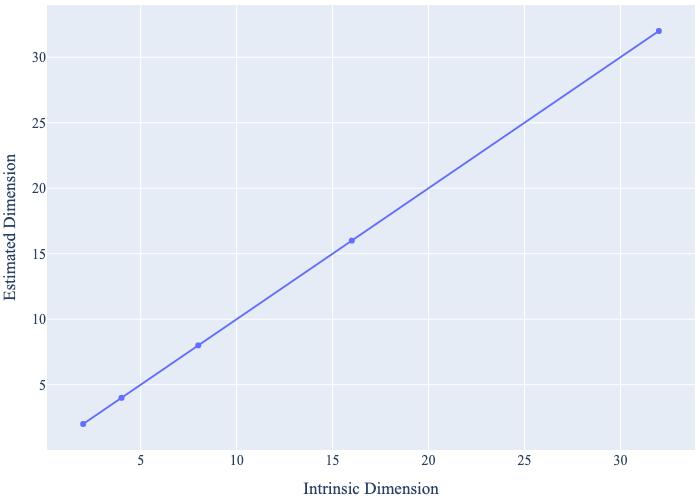
\includegraphics[width=\linewidth]{images/q5/gaussian.png}
        \caption{Intrinsic Dimension Estimation for Gaussian}
    \end{figure}

    \begin{figure}[h]
        \label{fig:hypercube_intrinsic_dim} 
        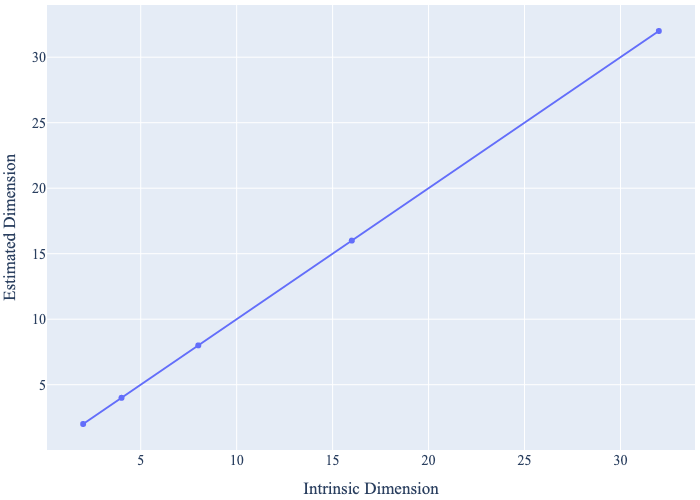
\includegraphics[width=\linewidth]{images/q5/hypercube.png}
        \caption{Intrinsic Dimension Estimation for Hypercube}
    \end{figure}

    \clearpage

\section{Numerical Exploration of Johnson-Lindenstrauss Lemma}

    Recall the Johnson-Lindenstrauss Lemma:

    \textbf{Lemma:} For $0<\epsilon<1$, set $X= \{ x_1 \ldots x_m \}$ with $x_i \in \mathbb{R}^N$, and $ n > 8 \ln(m)/ \epsilon^2$ there exists a linear map $f: \mathbb{R}^N \rightarrow \mathbb{R}^n$ such that:

    \begin{align*}
        (1 - \epsilon) ||u - v||^2 \leq ||f(u) - f(v)||^2 \leq (1 + \epsilon) ||u - v||^2
    \end{align*}

    for all $u,v \in X$.

    Furthermore, the linear map that satisifies this condition is given by $A \in \mathbb{R}^{n \times N}$ where $A_{ij} \sim \mathcal{N}(0, 1/n)$.

    To test this out numerically, I simulated the original data $X$, a projection matrix $A$, and then actually projected the data to $AX$.
    
    By the JL Lemma, we expect the distortion of distances to be bounded. Thus, for every pair of points $u, v \in X$, I computed the lower bound $(1-\epsilon) ||u - v||^2$, the upper bound $(1 + \epsilon) ||u-v||^2$, and the true distortion $||Au - Av||^2$. I numerically confirmed that the true distortion is between the upper and lower bounds for all pairs of points $u,v \in X$. I then plotted these distortion values to visually demonstrate this result: on the vertical axis, the embedding distortion (in black) falls between the upper and lower distortion bounds (in blue).

    \begin{figure}[h]
        \label{fig:jl_distortion} 
        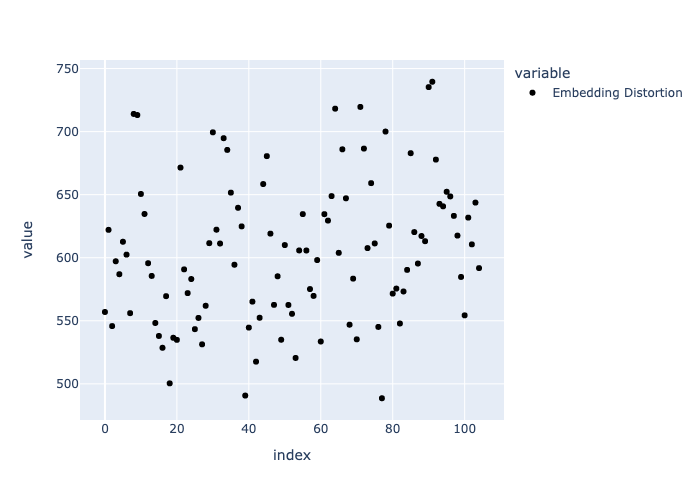
\includegraphics[width=1.3\linewidth]{images/q6/distortion.png}
        \caption{Distortion of Distances for JL Lemma}
    \end{figure}

    \clearpage

\end{document}